\documentclass[journal,12pt,twocolumn]{IEEEtran}
\usepackage{setspace}
\usepackage{gensymb}
\usepackage{xcolor}
\usepackage{caption}
\singlespacing
\usepackage{siunitx}
\usepackage[cmex10]{amsmath}
\usepackage{mathtools}
\usepackage{hyperref}
\usepackage{amsthm}
\usepackage{mathrsfs}
\usepackage{txfonts}
\usepackage{stfloats}
\usepackage{cite}
\usepackage{cases}
\usepackage{subfig}
\usepackage{longtable}
\usepackage{multirow}
\usepackage{enumitem}
\usepackage{bm}
\usepackage{mathtools}
\usepackage{listings}
\usepackage{tikz}
\usetikzlibrary{shapes,arrows,positioning}
\usepackage{circuitikz}
\renewcommand{\vec}[1]{\boldsymbol{\mathbf{#1}}}
\DeclareMathOperator*{\Res}{Res}
\renewcommand\thesection{\arabic{section}}
\renewcommand\thesubsection{\thesection.\arabic{subsection}}
\renewcommand\thesubsubsection{\thesubsection.\arabic{subsubsection}}

\renewcommand\thesectiondis{\arabic{section}}
\renewcommand\thesubsectiondis{\thesectiondis.\arabic{subsection}}
\renewcommand\thesubsubsectiondis{\thesubsectiondis.\arabic{subsubsection}}
\hyphenation{op-tical net-works semi-conduc-tor}

\lstset{
language=Python,
frame=single, 
breaklines=true,
columns=fullflexible
}
\begin{document}
\theoremstyle{definition}
\newtheorem{theorem}{Theorem}[section]
\newtheorem{problem}{Problem}
\newtheorem{proposition}{Proposition}[section]
\newtheorem{lemma}{Lemma}[section]
\newtheorem{corollary}[theorem]{Corollary}
\newtheorem{example}{Example}[section]
\newtheorem{definition}{Definition}[section]
\newcommand{\BEQA}{\begin{eqnarray}}
\newcommand{\EEQA}{\end{eqnarray}}
\newcommand{\define}{\stackrel{\triangle}{=}}
\newcommand{\myvec}[1]{\ensuremath{\begin{pmatrix}#1\end{pmatrix}}}
\newcommand{\mydet}[1]{\ensuremath{\begin{vmatrix}#1\end{vmatrix}}}
\bibliographystyle{IEEEtran}
\providecommand{\nCr}[2]{\,^{#1}C_{#2}} % nCr
\providecommand{\nPr}[2]{\,^{#1}P_{#2}} % nPr
\providecommand{\mbf}{\mathbf}
\providecommand{\pr}[1]{\ensuremath{\Pr\left(#1\right)}}
\providecommand{\qfunc}[1]{\ensuremath{Q\left(#1\right)}}
\providecommand{\sbrak}[1]{\ensuremath{{}\left[#1\right]}}
\providecommand{\lsbrak}[1]{\ensuremath{{}\left[#1\right.}}
\providecommand{\rsbrak}[1]{\ensuremath{{}\left.#1\right]}}
\providecommand{\brak}[1]{\ensuremath{\left(#1\right)}}
\providecommand{\lbrak}[1]{\ensuremath{\left(#1\right.}}
\providecommand{\rbrak}[1]{\ensuremath{\left.#1\right)}}
\providecommand{\cbrak}[1]{\ensuremath{\left\{#1\right\}}}
\providecommand{\lcbrak}[1]{\ensuremath{\left\{#1\right.}}
\providecommand{\rcbrak}[1]{\ensuremath{\left.#1\right\}}}
\theoremstyle{remark}
\newtheorem{rem}{Remark}
\newcommand{\sgn}{\mathop{\mathrm{sgn}}}
\newcommand{\rect}{\mathop{\mathrm{rect}}}
\newcommand{\sinc}{\mathop{\mathrm{sinc}}}
\providecommand{\abs}[1]{\left\vert#1\right\vert}
\providecommand{\res}[1]{\Res\displaylimits_{#1}} 
\providecommand{\norm}[1]{\left\Vert#1\right\Vert}
\providecommand{\mtx}[1]{\mathbf{#1}}
\providecommand{\mean}[1]{E\left[ #1 \right]}
\providecommand{\fourier}{\overset{\mathcal{F}}{ \rightleftharpoons}}
\providecommand{\ztrans}{\overset{\mathcal{Z}}{ \rightleftharpoons}}
\providecommand{\system}[1]{\overset{\mathcal{#1}}{ \longleftrightarrow}}
\newcommand{\solution}{\noindent \textbf{Solution: }}
\providecommand{\dec}[2]{\ensuremath{\overset{#1}{\underset{#2}{\gtrless}}}}
\let\StandardTheFigure\thefigure
\def\putbox#1#2#3{\makebox[0in][l]{\makebox[#1][l]{}\raisebox{\baselineskip}[0in][0in]{\raisebox{#2}[0in][0in]{#3}}}}
     \def\rightbox#1{\makebox[0in][r]{#1}}
     \def\centbox#1{\makebox[0in]{#1}}
     \def\topbox#1{\raisebox{-\baselineskip}[0in][0in]{#1}}
     \def\midbox#1{\raisebox{-0.5\baselineskip}[0in][0in]{#1}}

\vspace{3cm}
\title{Circle Assignment}
\author{Gautam Singh}
\maketitle
\bigskip

\begin{abstract}
    This document contains the solution to Question 12 of 
    Exercise 5 in Chapter 10 of the class 9 NCERT textbook.
\end{abstract}

\begin{enumerate}
    \item Prove that a cyclic paralellogram is a rectangle.

    \solution Consider the points $\vec{P_i},\ 1 \le i \le 4$ in anticlockwise 
    order on the unit circle. Thus, for $1 \le i \le 4$,
    \begin{align}
        \vec{P_i} = \myvec{\cos\theta_i\\\sin\theta_i} 
        \label{eq:circ-point}
    \end{align}
    where 
    \begin{align}
        \theta_i \in [0,2\pi),\ i \neq j \iff \theta_i \neq \theta_j
        \label{eq:theta-cond}
    \end{align}
    Without loss of generality, suppose that $P_1P_2$ and $P_3P_4$ are parallel 
    to the $x$-axis. Since
    \begin{align}
        \vec{P_1}-\vec{P_2} &= \myvec{\cos\theta_1-\cos\theta_2\\\sin\theta_1-\sin\theta_2} \\
        \vec{P_3}-\vec{P_4} &= \myvec{\cos\theta_4-\cos\theta_4\\\sin\theta_3-\sin\theta_4}
    \end{align}
    we have
    \begin{align}
        \sin\theta_1-\sin\theta_2 &= 0 \\
        \implies \sin\frac{\theta_1-\theta_2}{2}\cos\frac{\theta_1+\theta_2}{2} &= 0
        \label{eq:x-par}
    \end{align}
    However, from \eqref{eq:theta-cond}, we see that
    \begin{align}
        \theta_1-\theta_2 &\in \brak{-2\pi,2\pi} \\
        \implies \sin\frac{\theta_1-\theta_2}{2} &\neq 0 \\
        \implies \cos\frac{\theta_1+\theta_2}{2} &= 0 \\
        \implies \theta_1+\theta_2 &\in \brak{\pi,3\pi}
        \label{eq:theta-12}
    \end{align}
    Similarly,
    \begin{align}
        \theta_3+\theta_4 \in \brak{\pi,3\pi}
        \label{eq:theta-34}
    \end{align}
    Since $P_1P_2P_3P_4$ is a parallelogram, its diagonals bisect each other. 
    Thus, using \eqref{eq:theta-12} and \eqref{eq:theta-34},
    \begin{align}
        \frac{\vec{P_1}+\vec{P_3}}{2} &= \frac{\vec{P_2}+\vec{P_4}}{2} \\
        \implies \vec{P_1}+\vec{P_3} &= \vec{P_2}+\vec{P_4} \\
        \implies \myvec{\cos\theta_1+\cos\theta_3\\\sin\theta_1+\sin\theta_3} &= \myvec{\cos\theta_2+\cos\theta_4\\\sin\theta_2+\sin\theta_4} \\
        \implies \cos\theta_1+\cos\theta_3 &= \cos\theta_2+\cos\theta_4 \\
                                           &= -\brak{\cos\theta_1+\cos\theta_3} \\
        \implies \cos\theta_1+\cos\theta_3 &= \cos\theta_2+\cos\theta_4 = 0
        \label{eq:cos-diag}
    \end{align}
    Using \eqref{eq:cos-diag}, \eqref{eq:theta-12} and \eqref{eq:theta-34}, we have
    \begin{align}
        \cos\theta_1 &= -\cos\theta_3 = \cos\theta_4 \\
        \cos\theta_2 &= -\cos\theta_4 = \cos\theta_3
        \label{eq:theta-14-23}
    \end{align}
    Thus,
    \begin{align}
        \vec{P_1} - \vec{P_4} &= \myvec{\cos\theta_1-\cos\theta_4\\\sin\theta_1-\sin\theta_4} \\
                              &= \myvec{0\\\sin\theta_1-\sin\theta_4}
                              \label{eq:p1p4}
    \end{align}
    Thus, from \eqref{eq:p1p4},
    \begin{align}
        &\brak{\vec{P_1}-\vec{P_2}}^\top\brak{\vec{P_1}-\vec{P_4}} \nonumber \\
        &= \myvec{\cos\theta_1-\cos\theta_2&0}\myvec{0\\\sin\theta_1-\sin\theta_4} = 0
        \label{eq:adj-perp}
    \end{align}
    From \eqref{eq:adj-perp}, we see that $P_1P_2 \perp P_1P_4$. Hence, $P_1P_2P_3P_4$ is
    a rectangle.

    The situation is demonstrated in Fig. \ref{fig:circle}, plotted by the Python
    code \texttt{codes/circle.py}. The various input parameters are shown in Table
    \ref{tab:param}.
    \begin{table}[!ht]
        \centering
        \begin{tabular}{|c|c|}
            \hline
            \textbf{Parameter} & \textbf{Value} \\
            \hline
            $r$ & 1 \\
            \hline
            $\theta_1$ & $\frac{\pi}{6}$ \\
            \hline
            $\theta_2$ & $\frac{5\pi}{6}$ \\
            \hline
            $\theta_3$ & $\frac{7\pi}{6}$ \\
            \hline
            $\theta_4$ & $\frac{11\pi}{6}$ \\
            \hline
        \end{tabular}
        \caption{Parameters used in the construction of Fig. \ref{fig:circle}.}
        \label{tab:param}
    \end{table}
    
    \begin{figure}[!ht]
        \centering
        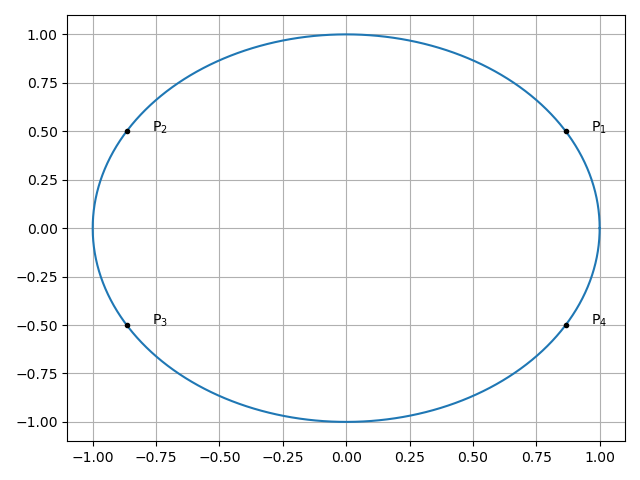
\includegraphics[width=\columnwidth]{figs/circle.png}
        \caption{$P_1P_2P_3P_4$ is a rectangle.}
        \label{fig:circle}
    \end{figure}
\end{enumerate}
\end{document}
